
Diese Hypothese geht davon aus, dass sich der Schnee durch mechanische Anregung von einem festen in den flüssigen Zustand übergeht.

Um die Idee zu testen, wird ein vibrierendes Objekt mit hoher Dichte auf den Schnee gelegt, und es wird beobachtet, wie sich das Objekt durch den Schnee bewegt.

Die Form des Objekts wurde vom AvaNode übernommen.  Ein Name, analog zum AvaNode, ist VibraNode. Fur die Umsetzung wurde ein Morphologischer Kasten mit drei Varinanten erstellt.


\begin{figure}[H]
    \centering
    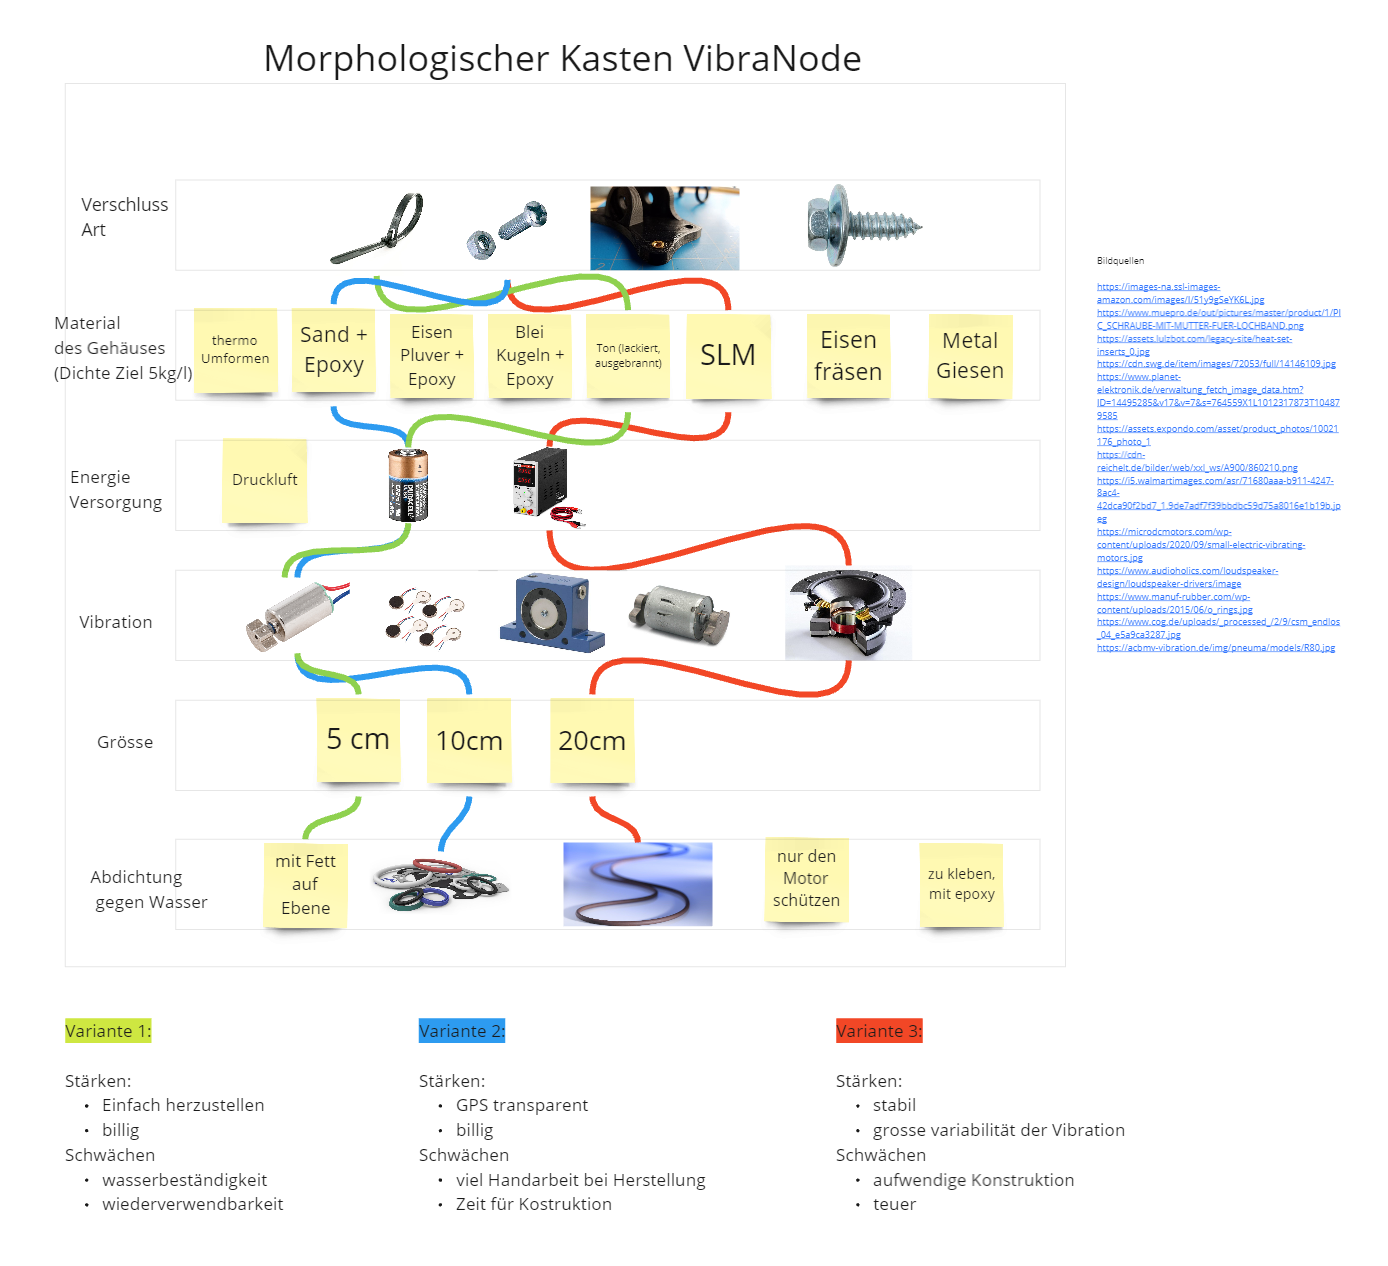
\includegraphics[width=0.8\textwidth]{Bilder/Unbenann2t.PNG}
    \caption{Morphologischer Kasten fur VibraNode}
    \label{fig:Bildverarbeitnugskonzpet}
\end{figure}


Um eine hohe Formfreiheit und eine hohe Dichte zu erreichen, habe ich den VibraNode aus Ton gebaut. Der ungebrannte Ton wurde durch Epoxy Harz und Acryl Farbe vor Wasser geschützt.

Die Testergebnisse fielen negativ aus. Der VibraNode konnte trotz seiner Dichte von 1600 kg/m3 nicht in den Schnee eindringen. Auch wenn der Schnee wurde mit flüssigem Wasser gesättigt und hat.  Damit  stellt sich die Frage, ob der LWC einen kausalen oder einen korrelativen Zusammenhang mit Gleitschneelawinen hat, und wie weit die Vorgeschichte des Schnees mitbetrachtet werden muss. \cite{Altman.2015}
